\begin{figure}
	\centering
	\begin{subfigure}{0.8\linewidth}
		\centering
		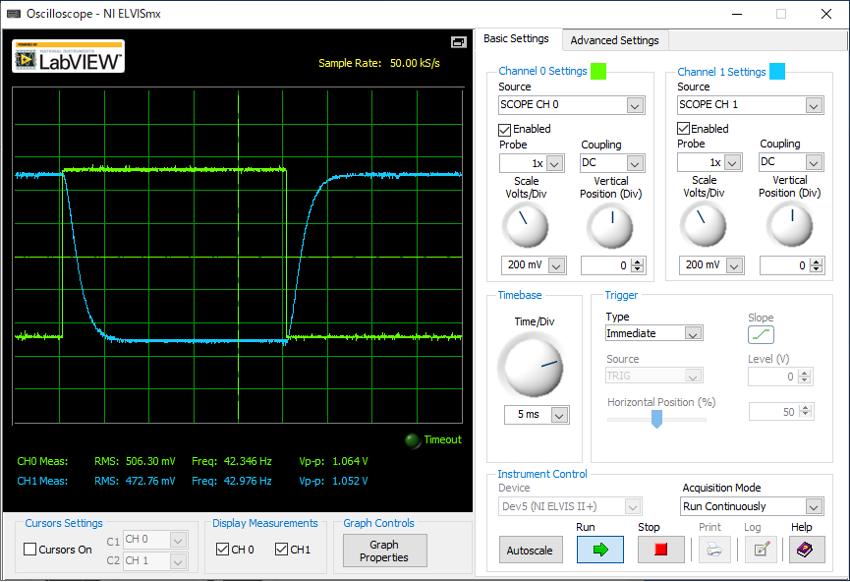
\includegraphics[width=0.8\linewidth]{src/figures/exp10/5k-low-sq.png}
		\subcaption{\SI{5}{k\ohm}でのバンドパスフィルタの出力波形}
	\end{subfigure}
	\begin{subfigure}{0.8\linewidth}
		\centering
		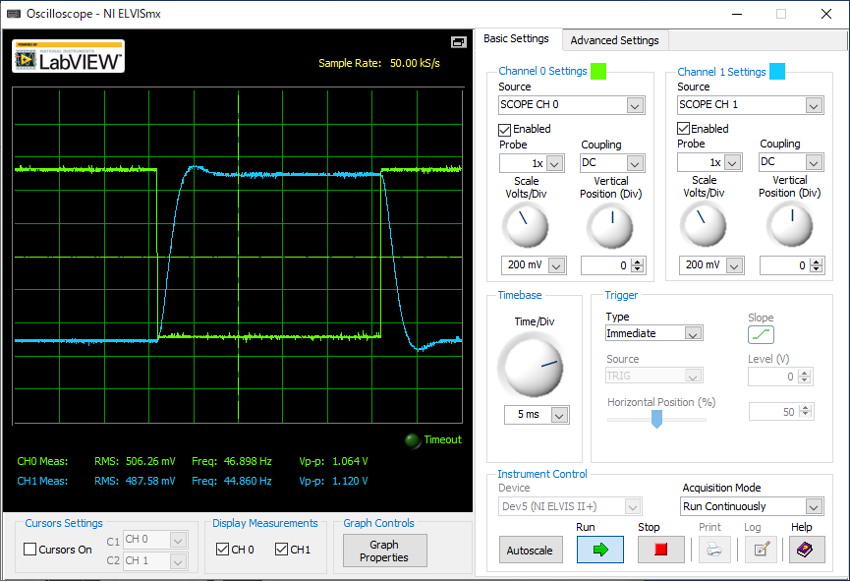
\includegraphics[width=0.8\linewidth]{src/figures/exp10/7k-low-sq.png}
		\subcaption{\SI{7}{k\ohm}でのバンドパスフィルタの出力}
	\end{subfigure}
\end{figure}
\begin{figure}
	\centering
	\begin{subfigure}{0.8\linewidth}
		\addtocounter{subfigure}{2}
		\centering
		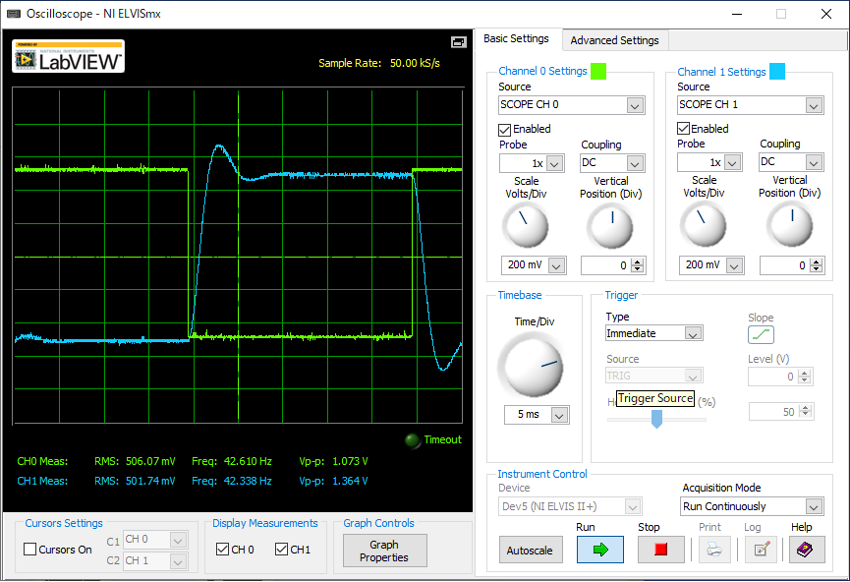
\includegraphics[width=0.8\linewidth]{src/figures/exp10/10k-low-sq.png}
		\subcaption{\SI{10}{k\ohm}でのバンドパスフィルタの出力波形}
	\end{subfigure}
	\begin{subfigure}{0.8\linewidth}
		\centering
		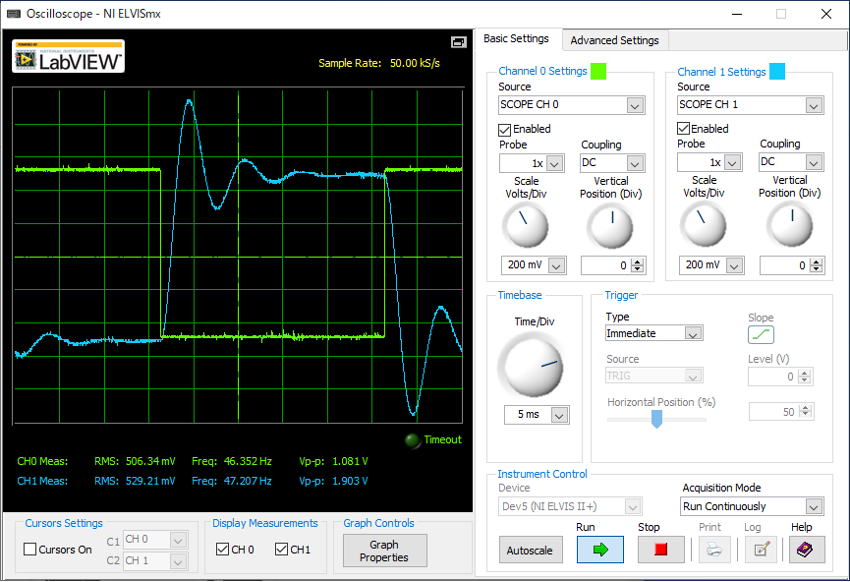
\includegraphics[width=0.8\linewidth]{src/figures/exp10/20k-low-sq.png}
		\subcaption{\SI{20}{k\ohm}でのバンドパスフィルタの出力波形}
	\end{subfigure}
	\caption{バンドパスフィルタの出力波形}
	\label{fig:exp10-band-sq}
\end{figure}
